\documentclass[9pt,twoside,lineno]{pnas-new}
% Use the lineno option to display guide line numbers if required.
\usepackage{rotating}
\templatetype{pnassupportinginfo}

\title{High geomagnetic field intensity recorded by anorthosite xenoliths requires a vigorous late Mesoproterozoic geodynamo}
\author{Yiming Zhang, Nicholas L. Swanson-Hysell, Margaret S. Avery, Roger R. Fu}
\correspondingauthor{Yiming Zhang\\E-mail: yimingzhang@berkeley.edu}

\begin{document}

\maketitle

%% Adds the main heading for the SI text. Comment out this line if you do not have any supporting information text.
% \SItext


% \subsection*{Subhead}
% Type or paste text here. This should be additional explanatory text such as an extended technical description of results, full details of mathematical models, etc.   

% \section*{Heading}
% \subsection*{Subhead}
% Type or paste text here. You may break this section up into subheads as needed (e.g., one section on ``Materials'' and one on ``Methods'').

% \subsection*{Materials}
% Add a materials subsection if you need to.

% \subsection*{Methods}
% Add a methods subsection if you need to.


\begin{figure*}[h!]
\noindent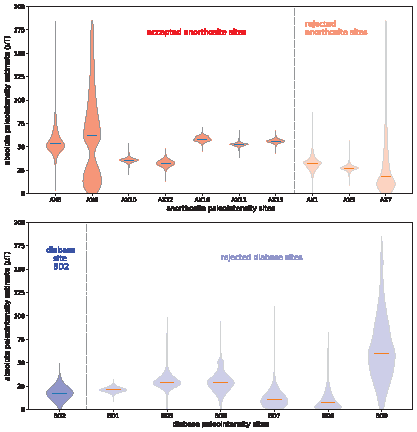
\includegraphics[width=17.8 cm]{manuscript/PINT_BiCEP.pdf}
\centering
\caption{{Violin plots of site-level posterior paleointensity distributions estimated using the bias corrected estimation of paleointensity (BiCEP) method developed by ref. \ref{Cych2021a}. Assuming that paleointensity estimates from specimens that come from a same cooling unit are distributed around a true paleointensity value with the various deflections being expressed as the curvature parameter of the NRM/TRM plot \cite{Arai1963a, Paterson2011a}, the method uses all paleointensity measurement-level data without applying selection criteria. For comparison of results from this independent method with those based on our selection (as show in Fig. 4 in manuscript), we highlight the anorthosite sites that pass our paleointensity selection and make other anorthosite and diabase transparent. The results from the BiCEP method address the uncertainties associated with anorthosite AX6 and AX8. This is associated with the relatively variable specimen behaviors within these two sites. But for sites AX10, AX11, AX13, AX12, and AX16, the posterior probability distributions have very narrow bounds, consistent with the interpretation that these anorthosites are faithful paleointensity recorders that have high-quality paleointensity behaviors. }}
\label{fig:PINT_BiCEP}
\end{figure*}

\clearpage

\begin{figure}
\noindent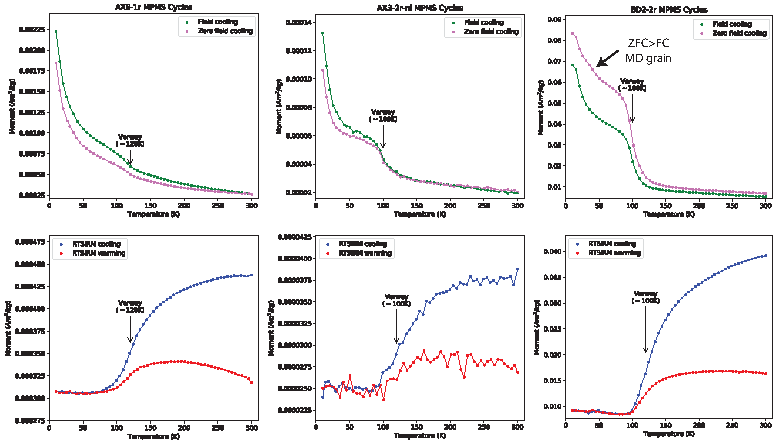
\includegraphics[width=\textwidth]{MPMS.pdf}
\centering
\caption{{Low-temperature magnetic property measurement system (MPMS) experiment results. In the field-cooled (FC) experiments, the magnetization was measured upon warming following the specimen having cooled in an applied field of 2.5 T from 300 to 10 K. In the zero-field-cooled (ZFC) experiment, a low-temperature saturation isothermal remanence (LTSIRM) of 2.5 T was applied at 10 K after the specimen cooled in a (near-)zero field. In the room-temperature saturation isothermal remanence (RTSIRM) experiment, the sample was pulsed with a 2.5 T field at room temperature ($\sim$300 K) and then cooled to 10 K and warmed back to room temperature in a (near-) zero field. Specimen AX6-1r is from anorthosite AX6 which passed our paleointensity selection. It has a well-defined Verwey transition $\sim$120 K \cite{Verwey1939a}. Specimens AX3-2r-ni and BD2-2r show Verwey transition but the transition temperatures are suppressed below $\sim$120 K. Specimen BD2-2r has a consistently higher moment during the zero-field-cooled step than during the field-cooled step. This is consistent with the interpretation that multidomian magnetic carriers exist in significant quantity in this specimen.}}
\label{fig:MPMS}
\end{figure}

\clearpage

\begin{figure*}[h!]
\noindent\includegraphics[width=17.8 cm]{Cooling_rate_correction.pdf}
\centering
\caption{{Graph of predicted paleointensity overestimate due to slow cooling of the intrusive Beaver River diabase and anorthosite xenoliths relative to the cooling rate in laboratory following the model of \citeA{Halgedahl1980a}. Because the majority of the anorthosites have unblocking temperatures between 500\textdegree C and 580\textdegree C, we estimate that the slow cooling during natural remanence acquisition could have resulted in a 36\% overestimate. Thus, a correction factor of 0.74 is applied at specimen level for the paleointensity summary plot.  }}
\label{fig:PINT_cooling_corrected}
\end{figure*}

\clearpage

% \begin{figure*}[h!]
% \noindent\includegraphics[width=17.8 cm]{.pdf}
% \centering
% \caption{{}}
% \label{fig:nonlinear_check}
% \end{figure*}

% \clearpage


\begin{sidewaystable}
\caption{\footnotesize{Summary paleointensity results for specimens that passed our selection. Paleointensity results for specimens that passed quality criteria. B$_{anc}$ is the calculated ancient field intensity over the chosen temperature interval in $\mu$T. T$_{min}$ and T$_{max}$ indicate the temperature interval over which the best fit for paleointensity was defined. N is the number of steps used within the selected interval for paleointensity determination. FRAC is the fraction of remanence. NpTRM shows the number of pTRM checks within the selected interval for paleointensity determination. $\beta$ is the scatter parameter.  GAP-MAX is the maximum magnetization gap between two adjacent steps. MAD is the maximum angle of deviation. DANG is the deviation angle. SCAT is the scatter parameter. Paleolatitude is calculated from the inclination values reported in \cite{Zhang2021b}. $\gamma$ is the gamma statistic that measures the angle between the last pTRM step used for paleointensity determination and the applied field direction. V(A)DM is the virtual (axial) dipole moment reported in $10^{21}$Am$^2$ (ZAm$^2$). }}
\centering
\begin{tabular}{cccccccccccccccc}
\hline
Site & Specimen & B$_{anc}$ & T$_{min}$ & T$_{max}$ & N    & FRAC & NpTRM & $\beta$ & GAP-MAX & MAD ($^\circ$) & DANG ($^\circ$) & SCAT & Paleolatitude & $\gamma$ & VADM (ZAm$^2$) \\
\hline
AX6  & AX6-2a   & 18.25     & 400       & 585       & 18 & 0.7  & 10.0  & 0.04    & 0.12    & 3.44           & 3.43            & PASS & 15.61         & 2.7      & 31.69          \\
AX6  & AX6-3a   & 25.39     & 400       & 585       & 18 & 0.76 & 10.0  & 0.04    & 0.1     & 4.28           & 2.88            & PASS & 15.61         & 3.2      & 44.08          \\
AX6  & AX6-1a   & 49.13     & 425       & 585       & 17 & 0.71 & 10.0  & 0.03    & 0.14    & 4.45           & 0.96            & PASS & 15.61         & 2.0      & 85.3           \\
AX8  & AX8-3a   & 41.3      & 400       & 580       & 17 & 0.75 & 9.0   & 0.03    & 0.14    & 4.38           & 2.22            & PASS & 17.16         & 11.2     & 70.45          \\
AX8  & AX8-1a   & 66.18     & 450       & 570       & 13 & 0.68 & 8.0   & 0.06    & 0.18    & 4.54           & 2.37            & PASS & 17.16         & 7.0      & 112.88         \\
AX10 & AX10-1a  & 45.84     & 425       & 585       & 17 & 0.78 & 10.0  & 0.06    & 0.24    & 5.6            & 2.62            & PASS & 14.41         & 4.7      & 80.64          \\
AX10 & AX10-3a  & 48.01     & 425       & 585       & 17 & 0.69 & 10.0  & 0.04    & 0.24    & 4.02           & 1.56            & PASS & 14.41         & 5.8      & 84.45          \\
AX10 & AX10-2a  & 48.23     & 425       & 585       & 17 & 0.67 & 10.0  & 0.05    & 0.19    & 5.3            & 1.93            & PASS & 14.41         & 7.8      & 84.84          \\
AX11 & AX11-1a  & 73.29     & 425       & 560       & 10 & 0.67 & 6.0   & 0.08    & 0.21    & 5.28           & 2.54            & PASS & 12.27         & 5.9      & 131.75         \\
AX11 & AX11-2a  & 73.29     & 400       & 560       & 11 & 0.65 & 6.0   & 0.07    & 0.21    & 3.94           & 1.51            & PASS & 12.27         & 9.9      & 131.75         \\
AX11 & AX11-4a  & 73.31     & 500       & 570       & 11 & 0.66 & 8.0   & 0.09    & 0.2     & 1.53           & 3.27            & PASS & 12.27         & 5.6      & 131.78         \\
AX11 & AX11-6a  & 73.32     & 200       & 562       & 14 & 0.69 & 7.0   & 0.07    & 0.17    & 4.0            & 1.33            & PASS & 12.27         & 3.0      & 131.8          \\
AX11 & AX11-9a  & 73.34     & 100       & 562       & 15 & 0.67 & 7.0   & 0.06    & 0.17    & 5.34           & 1.13            & PASS & 12.27         & 11.9     & 131.84         \\
AX11 & AX11-3a  & 73.41     & 400       & 560       & 11 & 0.66 & 6.0   & 0.08    & 0.21    & 3.95           & 2.11            & PASS & 12.27         & 8.2      & 131.96         \\
AX11 & AX11-5a  & 73.44     & 400       & 566       & 14 & 0.73 & 8.0   & 0.05    & 0.18    & 2.93           & 0.85            & PASS & 12.27         & 1.9      & 132.02         \\
AX12 & AX12-14a & 30.34     & 475       & 585       & 16 & 0.75 & 10.0  & 0.06    & 0.17    & 1.74           & 0.55            & PASS & 24.54         & 0.9      & 47.18          \\
AX12 & AX12-1a  & 33.89     & 0         & 580       & 21 & 0.97 & 9.0   & 0.03    & 0.17    & 5.47           & 4.73            & PASS & 24.54         & 10.0     & 52.7           \\
AX12 & AX12-6a  & 37.18     & 425       & 564       & 12 & 0.69 & 7.0   & 0.08    & 0.22    & 3.64           & 2.05            & PASS & 24.54         & 5.0      & 57.81          \\
AX12 & AX12-8a  & 38.34     & 475       & 565       & 12 & 0.75 & 8.0   & 0.06    & 0.25    & 1.46           & 2.29            & PASS & 24.54         & 1.6      & 59.62          \\
AX12 & AX12-4a  & 41.89     & 500       & 585       & 14 & 0.66 & 10.0  & 0.05    & 0.24    & 3.85           & 3.19            & PASS & 24.54         & 11.4     & 65.14          \\
AX12 & AX12-2a  & 46.94     & 425       & 570       & 14 & 0.7  & 8.0   & 0.05    & 0.24    & 3.39           & 2.38            & PASS & 24.54         & 7.0      & 72.99          \\
AX13 & AX13-3a  & 71.68     & 100       & 550       & 12 & 0.71 & 5.0   & 0.08    & 0.22    & 5.92           & 1.88            & PASS & 11.25         & 3.4      & 130.08         \\
AX13 & AX13-4a  & 75.42     & 200       & 555       & 12 & 0.7  & 6.0   & 0.03    & 0.17    & 7.28           & 0.41            & PASS & 11.25         & 3.7      & 136.87         \\
AX13 & AX13-6a  & 76.8      & 200       & 555       & 12 & 0.7  & 6.0   & 0.06    & 0.22    & 3.82           & 1.53            & PASS & 11.25         & 4.5      & 139.37         \\
AX13 & AX13-2a  & 76.96     & 300       & 555       & 11 & 0.69 & 6.0   & 0.05    & 0.2     & 7.87           & 2.73            & PASS & 11.25         & 4.1      & 139.66         \\
AX13 & AX13-9a  & 77.48     & 0         & 564       & 17 & 0.94 & 7.0   & 0.03    & 0.16    & 5.96           & 1.07            & PASS & 11.25         & 2.6      & 140.61         \\
AX13 & AX13-8a  & 84.83     & 450       & 570       & 13 & 0.81 & 8.0   & 0.02    & 0.24    & 3.69           & 1.82            & PASS & 11.25         & 5.1      & 153.94   \\
AX16 & AX16-13a & 41.68     & 400       & 570       & 15 & 0.72 & 8.0   & 0.07    & 0.2     & 3.47           & 1.85            & PASS & 22.11         & 1.1      & 66.88          \\
AX16 & AX16-16a & 42.2      & 400       & 570       & 15 & 0.77 & 8.0   & 0.06    & 0.15    & 3.9            & 1.81            & PASS & 22.11         & 2.0      & 67.72          \\
AX16 & AX16-14a & 43.57     & 400       & 570       & 15 & 0.71 & 8.0   & 0.06    & 0.13    & 3.25           & 1.79            & PASS & 22.11         & 6.0      & 69.91          \\
AX16 & AX16-11a & 44.17     & 450       & 570       & 14 & 0.7  & 8.0   & 0.06    & 0.15    & 2.86           & 2.07            & PASS & 22.11         & 4.6      & 70.88          \\
AX16 & AX16-5a  & 45.75     & 400       & 560       & 11 & 0.69 & 6.0   & 0.09    & 0.22    & 7.98           & 4.32            & PASS & 22.11         & 4.0      & 73.41          \\
AX16 & AX16-4a  & 45.96     & 425       & 570       & 14 & 0.75 & 8.0   & 0.05    & 0.21    & 5.01           & 1.18            & PASS & 22.11         & 4.2      & 73.75          \\
AX16 & AX16-2a  & 45.98     & 400       & 564       & 13 & 0.68 & 7.0   & 0.06    & 0.21    & 4.37           & 1.57            & PASS & 22.11         & 4.9      & 73.78          \\
AX16 & AX16-1a  & 46.25     & 200       & 562       & 14 & 0.85 & 7.0   & 0.07    & 0.23    & 6.04           & 2.87            & PASS & 22.11         & 4.5      & 74.22          \\
AX16 & AX16-9a  & 48.9      & 475       & 585       & 16 & 0.66 & 10.0  & 0.04    & 0.16    & 2.92           & 1.4             & PASS & 22.11         & 4.3      & 78.47          \\
AX16 & AX16-10a & 54.02     & 500       & 585       & 15 & 0.66 & 10.0  & 0.04    & 0.18    & 2.78           & 1.15            & PASS & 22.11         & 5.5      & 86.68          \\
\hline
\end{tabular}
\label{tab:PINT_result}
\end{sidewaystable}


\begin{table}

\caption{\footnotesize{Summary statistics for the Q$_{PI}$ quality criteria of \cite{Biggin2014a}.}}
\centering
\begin{tabular}{ccccccccccccc}
\hline
Site & N  & Age (Ma) & Method & AGE & STAT & TRM & ALT & MD & ACN & TECH & LITH & QPI \\ \hline
AX6  & 3  & 1091.8   & T+     & 1   & 0    & 1   & 1   & 1  & 1   & 0    & 0    & 5   \\
AX8  & 2  & 1091.8   & T+     & 1   & 0    & 1   & 1   & 1  & 1   & 0    & 0    & 5   \\
AX10 & 3  & 1091.8   & T+     & 1   & 0    & 1   & 1   & 1  & 1   & 0    & 0    & 5   \\
AX11 & 7  & 1091.8   & T+     & 1   & 1    & 1   & 1   & 1  & 1   & 0    & 0    & 6   \\
AX12 & 6  & 1091.8   & T+     & 1   & 1    & 1   & 1   & 1  & 1   & 0    & 0    & 6   \\
AX13 & 7  & 1091.8   & T+     & 1   & 1    & 1   & 1   & 1  & 1   & 0    & 0    & 6   \\
AX16 & 11 & 1091.8   & T+     & 1   & 1    & 1   & 1   & 1  & 1   & 0    & 0    & 6   \\ \hline
\end{tabular}
\label{tab:QPI}
\end{table}

% \begin{table}\centering
% \caption{This is a table}

% \begin{tabular}{lrrr}s
% Species & CBS & CV & G3 \\
% \midrule
% 1. Acetaldehyde & 0.0 & 0.0 & 0.0 \\
% 2. Vinyl alcohol & 9.1 & 9.6 & 13.5 \\
% 3. Hydroxyethylidene & 50.8 & 51.2 & 54.0\\
% \bottomrule
% \end{tabular}
% \end{table}

%%% Add this line AFTER all your figures and tables
\FloatBarrier

% \movie{Type legend for the movie here.}

% \movie{Type legend for the other movie here. Adding longer text to show what happens, to decide on alignment and/or indentations.}

% \movie{A third movie, just for kicks.}

% \dataset{dataset_one.txt}{Type or paste legend here.}

% \dataset{dataset_two.txt}{Type or paste legend here. Adding longer text to show what happens, to decide on alignment and/or indentations for multi-line or paragraph captions.}

\bibliography{YZ_ref}

\end{document}
